\documentclass{article}
\usepackage{amssymb}
\usepackage{courier}
\usepackage{fancyhdr}
\usepackage{fancyvrb}
\usepackage[T1]{fontenc}
\usepackage[top=.75in, bottom=.75in, left=.75in,right=.75in]{geometry}
\usepackage{graphicx}
\usepackage{lastpage}
\usepackage{listings}
\lstset{basicstyle=\small\ttfamily}
\usepackage{mdframed}
\usepackage{parskip}
\usepackage{ragged2e}
\usepackage{soul}
\usepackage{upquote}
\usepackage{xcolor}

% http://www.monperrus.net/martin/copy-pastable-ascii-characters-with-pdftex-pdflatex
\lstset{
upquote=true,
columns=fullflexible,
literate={*}{{\char42}}1
         {-}{{\char45}}1
         {^}{{\char94}}1
}

% http://tex.stackexchange.com/questions/40863/parskip-inserts-extra-space-after-floats-and-listings
\lstset{aboveskip=6pt plus 2pt minus 2pt, belowskip=-4pt plus 2pt minus 2pt}

\usepackage[colorlinks,urlcolor={blue}]{hyperref}

\begin{document}


\fancyfoot[L]{\color{gray} C4CS -- F'17}
\fancyfoot[R]{\color{gray} Revision 1.0}
\fancyfoot[C]{\color{gray} \thepage~/~\pageref*{LastPage}}
\pagestyle{fancyplain}

\title{\textbf{Advanced Homework 8\\}}
\author{\textbf{\color{red}{Due: Wednesday, November 8th, 11:59PM (Hard Deadline)}}}
\date{}
\maketitle


\section*{Submission Instructions}
To receive credit for this assignment you will need to stop by someone's
office hours, demo your running code, and answer some questions. \textbf{\color{red}{Make sure
to check the office hour schedule as the real due date is at the last office
hours before the date listed above.}} This applies to assignments that need to be gone over with a TA only.
\textbf{Extra credit is given for early turn-ins of advanced exercises. These details can be found on the website under the advanced homework grading policy.}


\begin{mdframed}[innerleftmargin=38pt,innerrightmargin=38pt]\justify
  For first two parts, you're welcome to keep going with the RPN example from
  lecture and the homework, \textbf{or} you may use code from one of your
  other EECS classes.

  {\color{red}Remember, you \textbf{MUST} use \textbf{PRIVATE} repositories
    for code from other EECS classes.} Private services are generally free for
  students, check out the \href{https://education.github.com/pack}{GitHub Student Developer Pack}.
\end{mdframed}

\section{Coverage}

Test suites are only as good as the code they test. If you don't test a
calculator's multiply function, then you will never notice if it breaks. The
term \emph{coverage} refers to how much of your code your tests cover---how
much is tested.

In addition to running your test suite, \emph{integration hooks} (the things
that run when you push changes to GitHub) can also do a test suite coverage
analysis. Some tools integrate with Travis, while others are standalone. I've
had success with Coveralls and Python, but you're welcome to try any code
coverage tool you like.

\textbf{Your job:} Add automated code coverage analysis to any project.

\subsection*{Submission checkoff:}
\begin{itemize}
  \item[$\square$] Which coverage tool did you use, why?
  \item[$\square$] What did you have to do to get the automatic integration
    working?
  \item[$\square$] Add some more code that you don't have a test for, show
    that coverage goes down.
    \begin{itemize}
      \item[$\square$] (You don't have to do this live, save a copy of an
        old report before adding new code)
    \end{itemize}
\end{itemize}

\section{A little vanity never hurt :)}

Maybe you've seen the little icons that show up on GitHub pages before that
report the status of tools:

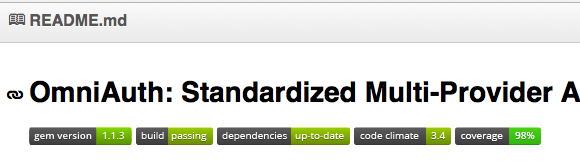
\includegraphics[width=.5\linewidth]{badges.png}

These are usually called \emph{badges}. They're a new-ish thing, but give a
nice at-a-glance status view for your project.

\subsection*{Submission checkoff:}
\begin{itemize}
  \item[$\square$] Add a badge for your build status from Travis CI
  \item[$\square$] If your coverage service supports badges (coveralls does),
    add that too
\end{itemize}


\section{Exploring Python's many libraries}

One of the things that makes Python very powerful is the diverse array of
\emph{modules} (the Python word for libraries) that it includes. For example,
it's annoying that in our calculator, if we have a typo, you can't just hit
the up arrow and edit the line, you have to type the whole thing again.

The bash terminal (and many, many other programs) use the \texttt{readline}
library for user input, and it provides many of the nicer things you're used
to (up arrow for last commands, Ctrl-r to search history, tab completion, etc).

By the magic of Python, we can get all those features really easily, simply
add the line:
\begin{quote}
  \texttt{import readline}
\end{quote}
near the top of your \texttt{rpn.py} file. Now when you run your calculator,
up arrow works!

\textbf{Your Job:} Find a Python library that does something cool and
integrate it into your calculator. (Or think of a cool feature you want and
find a Python library that does it!)

Some ideas:
\begin{itemize}
  \item Log smarter. Currently our calculator prints out its internal stack
    all the time, but really we only want to do that if we're debugging
    things.
  \item Colorize things. Print back the user input but highlight operators in
    a different color text. Maybe print negative numbers as a bold red.
  \item Handle errors better. Lots of unexpected inputs can kill the whole
    program, that's not great. Find something that will automatically recover
    and start again.
  \item If you're feeling adventurous, it's not too hard to create a basic
    graphical interface, number buttons and a text box, in Python
    (\href{https://wiki.python.org/moin/TkInter}{TkInter} is probably easiest,
    though not the prettiest -- there are
    \href{https://wiki.python.org/moin/GuiProgramming}{many options}).
  \item Or anything else you think is cool!
\end{itemize}

\subsection*{Submission checkoff:}
\begin{itemize}
  \item[$\square$] What new feature did you add?
  \item[$\square$] What module(s) did you use to make it happen?
\end{itemize}

\end{document}
